\documentclass[11pt,border=4pt]{standalone}
\usepackage{amsmath,amssymb,bm,mathtools}
\usepackage[fontset=fandol]{ctex}
\usepackage{tikz}
\usetikzlibrary{arrows.meta,calc,patterns,angles,quotes,decorations.markings,decorations.pathmorphing}
\newcommand{\dd}{\mathop{}\!\mathrm d}
\newcommand{\e}{\mathrm e}
\tikzset{axis/.style={->,>=Stealth,line width=.45pt},world/.style={line width=.8pt},flow/.style={->,>=Stealth,line width=.7pt},ray/.style={->,>=Stealth,line width=.7pt},guide/.style={dashed,line width=.35pt},aux/.style={dashed,line width=.35pt},dim/.style={<->,>=Stealth,line width=.35pt},every node/.style={font=\small},force/.style={->,>=Stealth,very thick},gas/.style={fill=blue!7}}
\begin{document}
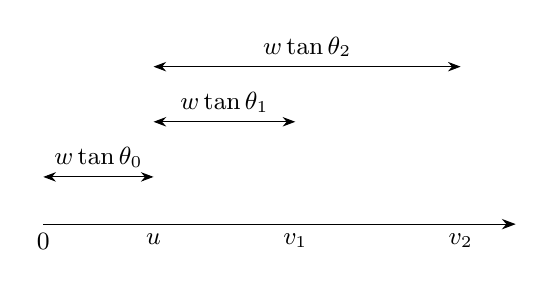
\begin{tikzpicture}\draw[axis](0,0)--(6,0);\node[below]at(0,0){$0$};\node[below]at(1.4,0){$u$};\node[below]at(3.2,0){$v_1$};\node[below]at(5.3,0){$v_2$};\draw[dim](0,.6)--(1.4,.6)node[midway,above]{$w\tan\theta_0$};\draw[dim](1.4,1.3)--(3.2,1.3)node[midway,above]{$w\tan\theta_1$};\draw[dim](1.4,2)--(5.3,2)node[midway,above]{$w\tan\theta_2$};\end{tikzpicture}
\end{document}
